% %%%%%%%%%%%%%%%%%%%%%%%%%%%%%%%%%%%%%%%%%%%%%%%%%%%%%%%%%%%%%%%%%%%%%
% %% State-of-the-Art %%
% OuterSPACE
% %%%%%%%%%%%%%%%%%%%%%%%%%%%%%%%%%%%%%%%%%%%%%%%%%%%%%%%%%%%%%%%%%%%%%

\subsection{OuterSPACE}
\label{sec:soa:outerspace}

OuterSPACE~\cite{Pal2018_OuterSPACE} is an \algo{OP} accelerator with a focus on SpMSpM kernels, although it can also handle SpMV. It is a highly parallelized architecture which employs Single-Program Multiple-Data (SPMD)-style \emph{processing elements} (\emph{PEs}) that fetch data from main memory through a two-level highly-banked cache hierarchy as shown in Figure~\ref{fig:soa:outerspace}. The input $A$- and $B$-matrices are stored in \emph{(UOP, CP) column-} and \emph{row-major} formats, respectively, to match the read access patterns of the \algo{OP} algorithm. The \emph{partial} and final outputs are stored in \emph{(UOP, CP)} format.

The computation is temporally divided into the \emph{multiply} and \emph{merge} phases (Figure~\ref{fig:soa:outerspaceHow}). During the first phase, inputs are divided into \emph{tiles} of several rows~($A$) and columns~($B$) and distributed through the \emph{processing tiles} (\emph{PTs}) by a \emph{control unit}. Within each \emph{PT}, each \emph{PE} processes multiplications of one element of the $k^{th}$ $A$-column with all elements of the $k^{th}$ $B$-row and an L0 cache in the \emph{PT} facilitates the reuse of the $B$-rows between \emph{PEs}. This phase generates a \emph{partial output} (\emph{PO}) per \emph{PT}, corresponding to the \emph{tile} of rows~($A$) and columns~($B$) that it was assigned.

Then, during the \emph{merge} phase, the \emph{POs} are combined to generate the final $C$-matrix. Each \emph{PT} locally sorts the \emph{POs}, and then the \emph{PTs} work together to merge them. This algorithm was chosen to maximize data locality and parallelism, although it is less efficient. This \emph{merge} phase only uses half of the \emph{PEs} so the others are disabled (clock-gated) and the caches are reconfigured in a scratchpad mode to save energy.

Note, if $NNZ$ elements in the \emph{POs} exceeds the L0 cache capacity, it overflows to the last level cache, which results in reduced performance. OuterSPACE performs best when the $NNZ_c(A)$ and $NNZ_r(B)$ are both uniform which ensures a uniform distribution of work across the large number of \emph{PTs} and \emph{PEs}.

\begin{figure}
    \centering
    \begin{minipage}[b]{0.49\linewidth}
        \begin{figure}[H]
            \centering
            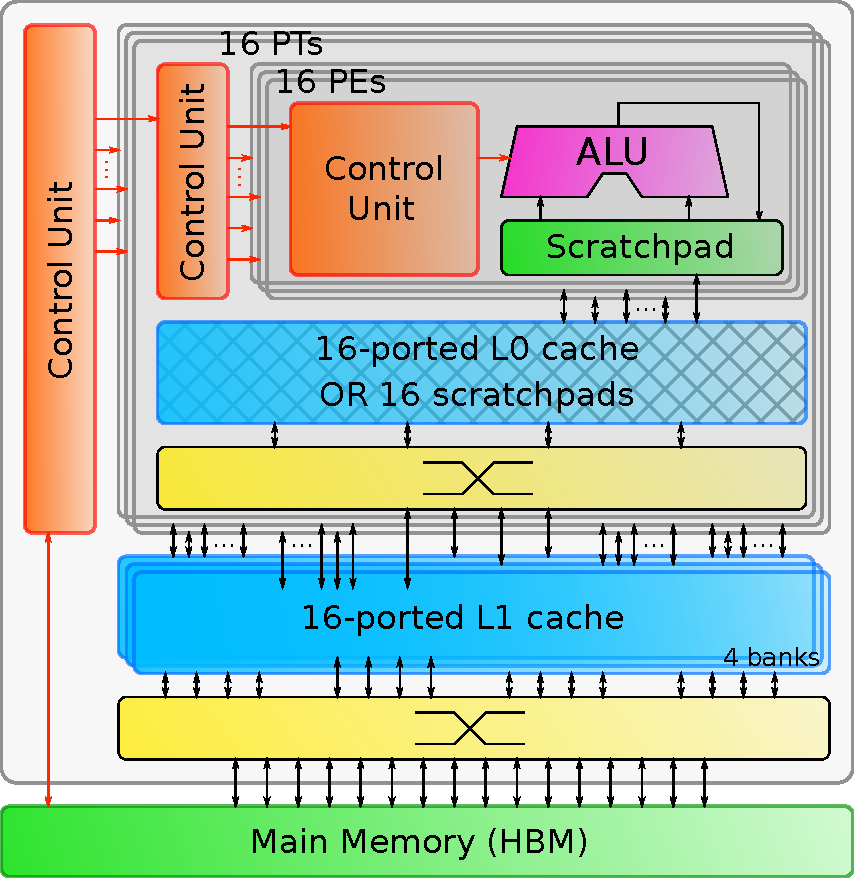
\includegraphics[width=0.7\textwidth]{Chapter_SoA/Figures/PDF/OuterSPACE.pdf}
            \caption{Architecture of OuterSPACE}
            \label{fig:soa:outerspace}
        \end{figure}
    \end{minipage}
    \hfill
    \begin{minipage}[b]{0.49\linewidth}
        \begin{figure}[H]
            \centering
            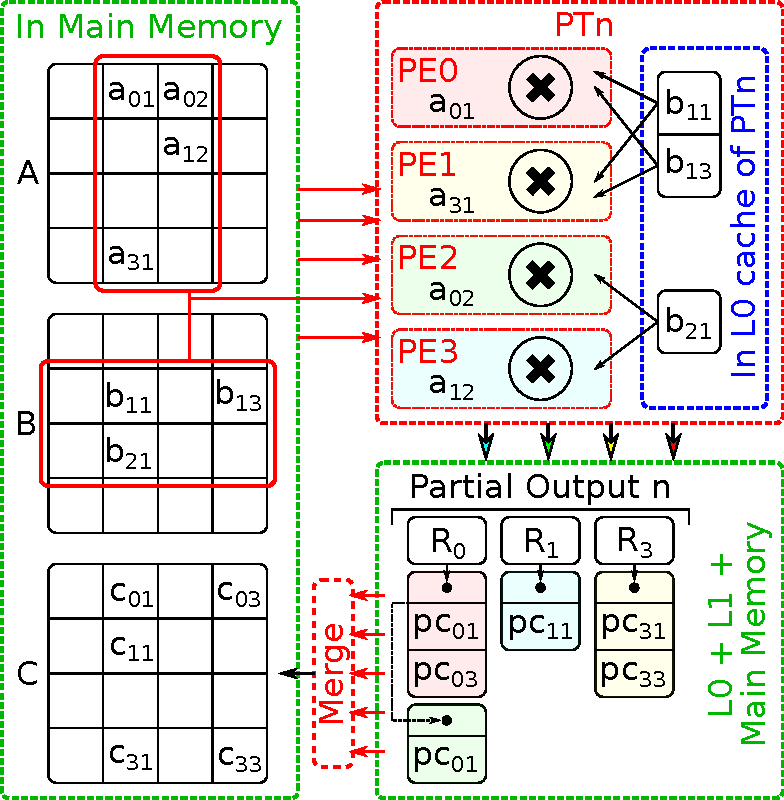
\includegraphics[width=0.705\textwidth]{Chapter_SoA/Figures/PDF/OuterSPACE_How_Vertical.pdf}
            \caption{OuterSPACE Data Flow}
            \label{fig:soa:outerspaceHow}
        \end{figure}
    \end{minipage}
\end{figure}